\documentclass{beamer}
\usetheme{utk}
\usepackage{listings}
\lstdefinelanguage{algorithm}{
	morekeywords={for, while, to, downto, by, repeat-until, if, else, each, foreach, in},
	otherkeywords={=>,<-,<\%,<:,>:,\#,@},
	sensitive=true,
	morecomment=[l]{//},
	morecomment=[n]{},
	morestring=[b]",
	morestring=[b]',
	morestring=[b]"""
	keywordstyle=\color{blue}\bfseries,  
	escapeinside={`}{`}
}
\usepackage{graphicx}
\usepackage{amsmath}
\usepackage{amssymb}

\AtBeginSection[]
{
	\begin{frame}
		\frametitle{Outline}
		\tableofcontents[currentsection, subsectionstyle = show/shaded/hide, subsubsectionstyle = hide]
	\end{frame}
}

\AtBeginSubsection[]
{
	\begin{frame}
		\frametitle{Outline}
		\tableofcontents[currentsection, 
		subsectionstyle = show/shaded/hide, subsubsectionstyle = show/shaded/hide]
	\end{frame}
}
\AtBeginSubsubsection[]{
		\begin{frame}
		\frametitle{Outline}
		\tableofcontents[sectionstyle=hide, 
		currentsubsection,
		subsubsectionstyle = show/shaded/hide]
	\end{frame}
}



\title[Genetic Algorithms in Classification]{On the Role of Genetic Algorithms in the Pattern Recognition Task of Classification}
\author{Isaac Sherman}
\institute{Electrical Engineering and Computer Science}

\begin{document}

\begin{frame}
\titlepage
\end{frame}

\begin{frame}
	\frametitle{Outline}
	\tableofcontents
\end{frame}

\section{Introduction}
\begin{frame}[fragile]
\frametitle{Basic Genetic Algorithm}
\begin{lstlisting}[language = algorithm, basicstyle=\scriptsize]
BasicGA():
	Population := RandomInitialization()
	while True:
		for each Solution in Population:
			Evaluate Solution
			Assign Fitness to Solution
		newPopulation = SurviveAndBreed(Population)
		Population = newPopulation
	end while
	
	\end{lstlisting}
\end{frame}

\begin{frame}
	\frametitle{Example}
	Consider an equation of the form $$		a \: op_1\: b\: op_2\: c\: op_3\: d =x$$
	If we know x, we can use a GA to find operators and values which satisfy it.  For instance, 
	$$		3 \times 7 \times 3 + 5 = 68$$
	Each digit can be encoded with 4 bits, each operator with 2.  Values over 9 for digits are rerolled until valid.
\end{frame}
\begin{frame}[fragile]
	
	\frametitle{Operators for Example}
	\begin{tabular}{|c| c|}\hline
	Bits & Operator\\
	\hline
	00&$+$\\
	01&$-$\\
	10&$\times$\\
	11&$\div$\\
	\hline
\end{tabular}

Therefore, \\

\begin{tabular}{c c c c c c c}
	3& $\times$& 7& $\times$& 3& +& 5\\
	0011&11&1011&11&0011&00&0101\\
\end{tabular}
\end{frame}

\begin{frame}
	\frametitle{Example-> Fitness function}
	Here, we maximize $\frac{1}{|S_i-x|}$ and stop when $S_i = x$.\\
	So, if x is 72, then the fitness of $$3 \times 7 \times 3 + 5 = 68$$
	is $\frac{1}{|68-72|} = 0.25$
\end{frame}

\begin{frame} \frametitle{Motivation}
\begin{itemize}
	\item Where do GAs fit in the greater scheme of pattern recognition?
	\item Given primitive mechanics, can they match or exceed theoretically-based methods?
	\item Can we build a generic, universal genetic algorithm for classification?
\end{itemize}

\end{frame}
\section{Methodology}

\begin{frame}

\end{frame}

\subsection{Program Flow}

\begin{frame}
\begin{figure}
	\centering
	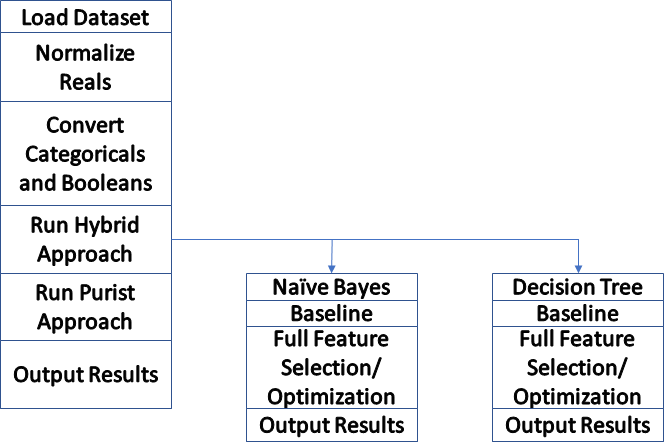
\includegraphics[width=0.7\linewidth]{figures/png/ProgramFlow}
	\caption[Overall Program Flow]{Birds-eye view of the flow of the program.
		Hybrid approaches are not run in parallel, because at time of coding MATLAB
		doesn't support multi-threading via a COM server.}
	\label{fig:ProgramFlow}
\end{figure}
\end{frame}
\begin{frame}
	\frametitle{For Reals}
	Categorical feature types:
	\begin{align*}
	X &= {X_\mathbb{R} \cup X_{cat} \cup X_{bool}}\\
	X_\mathbb{R} &= \{x_1, x_2, ... x_n\}\\
	X_{cat} &= \{x_{n+1}, x_{n+2}, ... x_c\}\\%there are some number of categorical columns,
	%each of which have a number of categoricals in them.
	X_{bool} &= \{x_{c+1}, x_{c+2,} ... x_b\} \\
	1&\leq i \leq c-n\\
	L &= \{x_i|x_i\epsilon X_{cat}\}\\%Set of categoricals
	C_\ell &= \{x, i|  x\epsilon X \wedge x_{n+i} = \ell\epsilon L \}\\%set of samples
	%belonging to categoricals
	R(\ell) &= \frac{\sum_{x\epsilon C_\ell}\sum_{j=1}^{n}x_j}{|C_\ell|n}
	\end{align*}
	
\end{frame}
\begin{frame}
	\frametitle{Booleans}
	True is converted to .75, false to .25.
\end{frame}


\subsection{Optimizers}
\begin{frame}
	\frametitle{Hybrid Approach}
	\begin{itemize}
		\item Optimizers are solutions which optimize, in this case, classifiers.
		\item Their purpose is to optimize which settings a classifier uses as well as selecting features.
		\item Each feature is represented as a bit, usually at the front of the Optimizer.
		\item The remainder of the genome represent parameters to the classifier
		\item Two classifiers, Na\"ive Bayes (McNB) and Classification Tree (CTree)
		\item Further, two versions of each: with and without feature selection (baseline)
		\item Fitness is defined as the average accuracy per class, or $\overline{A}$
	\end{itemize}
\end{frame}

\begin{frame}{Fitness}
	Consider C = \\\begin{tabular}{|c|c|c|c|c|}
		\hline
		True:&$\omega_1$&$\omega_2$&$\omega_3$&\textbf{Total}\\
		\hline
		Predicted $\omega_1$&4&6&5&\textbf{15}\\
		\hline
		Predicted $\omega_2$&2&2&9&\textbf{13}\\
		\hline
		Predicted $\omega_3$&8&2&110&\textbf{120}\\
		\hline
		Total&\textbf{14}&\textbf{10}&\textbf{124}&\textbf{148}\\
		TPR&0.286&0.20&0.89&.459\\
		\hline
	\end{tabular} 
\\In this case, $A$ = $\frac{4+2+110}{148} = 78.4\%$, but $\overline{A} = .459$, which better reflects its performance. 
%(MCC and CEN are 0.293 and 0.356, respectively)
\end{frame}

\subsubsection{Na\"ive Bayes}
\begin{frame}
	\frametitle{Na\"ive Bayes}
	\begin{equation*}
	P(\omega_j|x) = \frac{p(x|\omega_j)P(\omega_j)}{p(x)}
		\end{equation*}
	Where: \begin{itemize}
		\item $P(\omega_j|x)$ is the posterior probability that x belongs to class j
		\item $P(\omega_j)$ is the rate of occurrence of class j, called the prior probability.
		\item $p(x|\omega_j)$ is the likelihood of x belonging to $\omega_j$
		\item $p(x)$ is a normalizing constant to constrain values to $\epsilon[0,1]$
	\end{itemize}
	\vspace{2cm}
	
	\tiny{Shamelessly reproduced from Dr. Hairong Qi's ECE 471 slide}
\end{frame}
\begin{frame}
		\frametitle{Na\"ive Bayes}
		Optimizers optimize the following: 
		\begin{itemize}
			\item Features, 1 bit per feature
			\item Distribution, 2 bits
			\item Kernel, 2 bits
			\item Score Transform, 3 bits
			\item Priors, 3 bits per class
		\end{itemize}
\end{frame}

\begin{frame}
	\frametitle{Na\"ive Bayes}
	Distribution uses 2 bits and can be one of the following: 
	\begin{itemize}
	\item \textbf{Kernel} uses a smoothing function to build a distribution
	\item	\textbf{Multinomial} represents every class as a single multinomial distribution
	\item	\textbf{Multivariate multinomial} characterizes each feature as an independent multinomial distribution based on the unique values found in the feature.
	\item	\textbf{Normal}
	\end{itemize}
\end{frame}

\begin{frame}
	\frametitle{Na\"ive Bayes}
	Kernel uses 2 bits and can be one of the following: 
	\begin{itemize}
		\item \textbf{Box} uses a uniform, box-like smoothing window.
		\item \textbf{Epanechnikov} is a very efficient, rounded kernel.
		\item \textbf{Gaussian} is a standard normal function but used in this case for smoothing.
		\item \textbf{Triangular} is another form of smoothing, with a peak of 1 at 0 and zero at -1 and 1.
	\end{itemize}
\end{frame}
\begin{frame}{Na\"ive Bayes}
	Score transform uses 3 bits and can be any of the following:
\begin{itemize}
	\item \textbf{DoubleLogit} transforms the score to $\frac{1}{1+e^{-2x}}$
	\item \textbf{Invlogit} $log(\frac{x}{1-x})$
	\item \textbf{Logit} $\frac{1}{1+e^{-x}}$
	\item \textbf{None} $x$
	\item \textbf{Sign} $\frac{x}{|x|}$, or 0 when x = 0.
	\item \textbf{Symmetric} $2x-1$
	\item \textbf{Symmetricismax} 1 if max of class, 0 otherwise
	\item \textbf{Symmetriclogit} $\frac{2}{1+e^{-x}}-1$
\end{itemize}
\end{frame}

\subsubsection{Classification Tree}
	
\begin{frame}
	\frametitle{Classification Tree}
	  \begin{itemize}
	  	\item \textbf{Features}, 1 bit per feature
		\item \textbf{Merge Leaves},  1 bit
		\item \textbf{Maximum Splits}, 6 bits
		\item \textbf{Min Leaf Size}, 5 bits
		\item \textbf{Split Criterion}, 2 bits
	\end{itemize}
\end{frame}


\begin{frame}
	\frametitle{Classification Tree}
\textbf{Merge Leaves} takes 1 bit and is either on or off.  Merge leaves looks at leaves from a parent node and if the amount of their risk and that of their offspring is at or greater than that of a parent.\vspace{5mm}
\textbf{Maximum Splits} defines how many splits a tree can have.  The tree is built iteratively, layer by layer, splitting as needed until it hits this number.  It can take on values of 3-66.\\
\end{frame}
\begin{frame}{Classification Tree}
\textbf{Min Leaf Size} This is the minimum number of samples that need to reach this node to be considered a standalone leaf.  Beyond this number (specifically, at twice this number) a leaf become a parent node split into two children. Takes on values between 1 and 32.\\
\end{frame}

\begin{frame}{Classification Tree}
		\textbf{Split Criterion} can take on 3 values.
		\begin{itemize}
			\item \textbf{Gini's Diversity Index} Aims for maximally diverse cuts
			\item \textbf{Twoing} Aims for a balanced tree
			\item \textbf{Deviance} Minimizes entropy
		\end{itemize}
\end{frame}

\begin{frame}[fragile]
	\frametitle{Evolver}
	\begin{lstlisting}[language = algorithm, basicstyle=\scriptsize]
AdvanceGeneration():
	EvaluateAllOptimizers(P) //Multithreaded evaluation possible
	GetMetrics()
	P.ReverseSort()//P is the population, an instance variable
	P = GenerateNextGeneration(P)
	RemoveDuplicates(P)
	
GenerateNextGeneration(P):
	BreedingPop := StochasticRUS(P)
	NextGen := Elitism(P)
	FillListFromBreedingPop(NextGen, BreedingPop,
				P.Count, UniformXOver)
	MutateNonElites(NextGen)
	return NextGen
	\end{lstlisting}
\end{frame}

\begin{frame}[fragile]
	\frametitle{Evolver}
	\begin{lstlisting}[language = algorithm, basicstyle=\scriptsize]
	FillListFromBreedingPop(N, B, size, Func):
	E := B.Count * ElitePercent
	while(N.Count < size):
		k := j := RNG.Next(0, E)
		while(j==k) 
			k = RNG.Next(0, B.Count)
		for each offspring in Func(B[j], B[k])
		N.Add(offspring)
	
	while (N.Count > size)
		N.pop()
	\end{lstlisting}
	
\end{frame}

\subsection{Hunters}
\begin{frame}
	\frametitle{Hunters}
		\begin{itemize}
			\item Hunters are made up of 1 or more Chromosomes
		\item Chromosomes are made up of 1 or more Cells
		\item Cells form the bulk of the genome of the Hunter
		\item Fitness is a modified $\overline{A}$
	\end{itemize}
Examine each component from the bottom up
\end{frame}

\begin{frame}{Hunter Fitness}
	Fitness is equal to $\overline{A}$ with 2 scalars, one for complexity and one for ignoring classes:
	$$F_{Hunter} = \overline{A} \bigg( \frac{C_{Max} - C}{C_{Max}}\bigg) \bigg( \frac{E-Z}{E}\bigg)$$
	  
\end{frame}

\subsubsection{Component Structure}
\begin{frame}{Cells}

Cells comprise the following:
\begin{itemize}
	\item Function Index, \(\lceil log_2(F)\rceil\) bits, where F is the number of features
	\item Upper Limit, 8 bits
	\item Lower Limit, 8 bits
	\item Not Flag, 1 bit
	\item Join Bit, 1 bit
\end{itemize}
\end{frame}

\begin{frame}{Cells}
	\textbf{Functions} \((F_i)\) are simply looking at features, looking at the values of the normalized dataset.  \\
	\textbf{Limits} are a binary number shifted to the -8th power.  It allows for values between 0 and \(\frac{511}{512}\).  If the upper limit \((L_u)\) is lower than the lower limit\((L_\ell)\), the bits are swapped.\\
	The \textbf{Not Flag} (N) reverses the vote of the cell. \\
	So when a cell votes, it returns \(V= N\oplus  (L_\ell \leq F_i \leq L_u)\)\\ 
	The Join Bit indicates whether to include the next cell in the voting process. 
\end{frame}
\begin{frame}{Chromosomes}
	Chromosomes comprise the following:
\begin{itemize}
	\item Class Bits, \(\lceil log_2(\Omega)\rceil\) bits where \(\Omega\) is the number of classes
	\item Affinity Bits, 2
	\item A List of Cells
\end{itemize}
\end{frame}

\begin{frame}{Chromosomes}
	Chromosomes comprise the following:
	\begin{itemize}
		\item Class Bits, \(\lceil log_2(\Omega)\rceil\) bits where \(\Omega\) is the number of classes
		\item 2 Affinity Bits, discussed in detail later
		\item A List of Cells
	\end{itemize}
\end{frame}

\begin{frame}{Hunters}
	Hunters are merely a housing for a list of Chromosomes.  They don't contain any genetic information of their own.  However, breeding operations and fitness is calculated at the Hunter level.
\end{frame}
\subsubsection{Breeding Functions}
\begin{frame}{Crossover}
	Crossover functions differently because Hunters are of variable length.  It performs uniform crossover on the lengths which match, but then randomly assigns entire chromosomes to either offspring following the uniform crossover style.
	 
\end{frame}

\begin{frame}{Crossover}

\begin{figure}
	\centering
	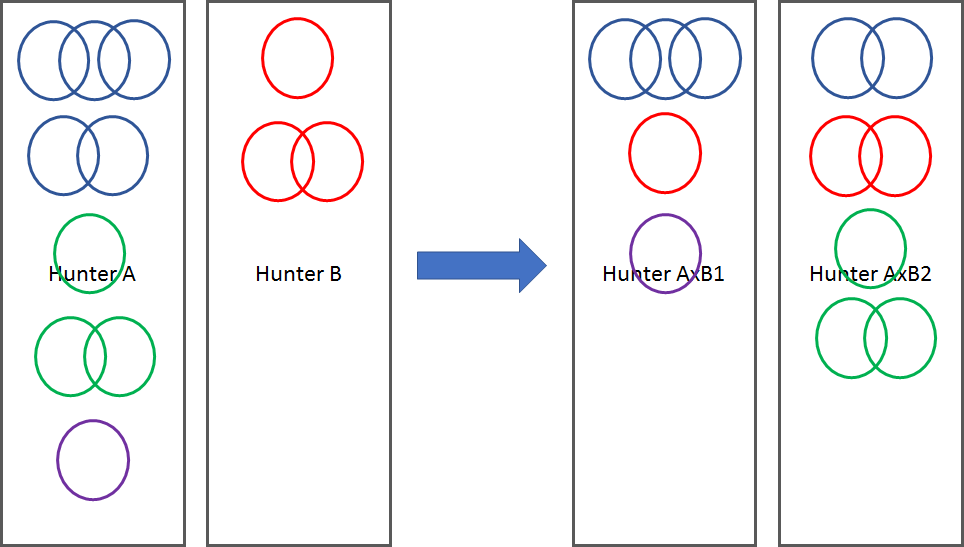
\includegraphics[width=0.7\linewidth]{figures/png/HunterCrossover}

	\label{fig:huntercrossover}
\end{figure}
\end{frame}

\begin{frame}{Merge}
	Merge takes 2 hunters and returns a single hunter with a combination of the material of both.  The action occurs mostly at the chromosomal level.  \\
	Chromosomes have 2 affinity bits which controls the merge operation.\\
	Individually, bits may be understood as follows:
	\centering
	\begin{tabular}{|c c | l|}
		\hline
		 &  & Meaning \\
		\hline
		0 & 0 & No preference.\\
		0 & 1 & Prefers to be at the rear.\\
		1 & 0 & Prefers to be at the front.\\
		1 & 1 & Considers itself complete.\\
		\hline
	\end{tabular}\\
	 
	
\end{frame}
\begin{frame}
	When two chromosomes go to merge, the results are determined as follows:\\
		\centering
	\begin{tabular}{|c c | l|}
		\hline
		A & B & Result\\
		\hline
		%start with horizontal, A first
		00 & 00 & \\
		00 & 01 &\\
		10 & 00 &\\
		10 & 01 &Laid out Horizontally with A in front\\
		\hline
		00 & 10&\\
		01 & 00&\\
		01 & 10& Laid out Horizontally with B in front\\
		\hline
		11 & ** & \\
		** & 11 & \\
		10 & 10 & \\
		01 & 01 & Laid out Vertically\\
		\hline	
	\end{tabular}
	
\end{frame}
\begin{frame}{Merge}
	
	\begin{figure}
		\centering
		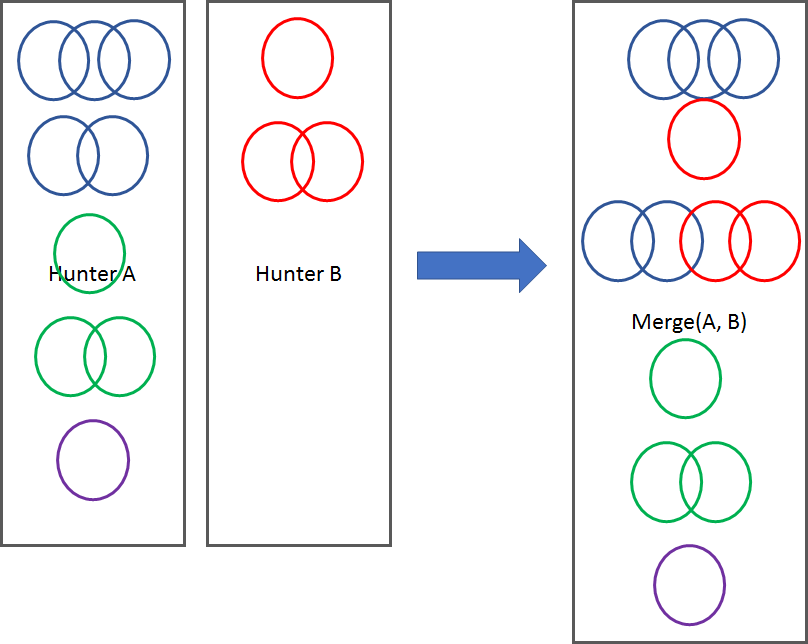
\includegraphics[width=0.7\linewidth]{figures/png/HunterMerge}
		
		\label{fig:huntermerge}
	\end{figure}
\end{frame}


\subsection{Metrics}
\begin{frame}{Metrics}
	Matthews Correlation Coefficient (MCC) and Confusion Entropy (CEN) are two promising additional methods for analyzing confusion matrices.
	$$MCC = \frac{cov(X,Y)}{\sqrt{cov(X,X)\cdot cov(Y,Y)}}$$
	\begin{itemize}
		\item Falls in the range  [-1,1]
		\item 1 indicates perfect classifier
		\item -1 indicates perfect anti-classifier
		\item 0 indicates one or more columns is equal to 0
	\end{itemize}
\end{frame}
\begin{frame}{Metrics}
	Consider C = \\\begin{tabular}{|c|c|c|c|c|}
		\hline
		True:&$\omega_1$&$\omega_2$&$\omega_3$&\textbf{Total}\\
		\hline
		Predicted $\omega_1$&4&6&5&\textbf{15}\\
		\hline
		Predicted $\omega_2$&2&2&9&\textbf{13}\\
		\hline
		Predicted $\omega_3$&8&2&110&\textbf{120}\\
		\hline
		Total&\textbf{14}&\textbf{10}&\textbf{124}&\textbf{148}\\
		TPR&0.286&0.20&0.89&.459\\
		\hline
	\end{tabular} 
	\\In this case, $A$ = $\frac{4+2+110}{148} = 78.4\%$, but $\overline{A} = .459$, which better reflects its performance. 
	%(MCC and CEN are 0.293 and 0.356, respectively)
\end{frame}

\section{Results}
\subsection{Yeast}
\subsection{Cardiotocography}
\subsection{Bach's Chorales}

\section{Discussion}
\end{document}
